\documentclass[journal,12pt,twocolumn]{IEEEtran}

\usepackage{setspace}
\usepackage{gensymb}
\singlespacing
\usepackage[cmex10]{amsmath}

\usepackage{amsthm}
\usepackage{mathrsfs}
\usepackage{txfonts}
\usepackage{stfloats}
\usepackage{bm}
\usepackage{cite}
\usepackage{cases}
\usepackage{subfig}

\usepackage{longtable}
\usepackage{multirow}

\usepackage{enumitem}
\usepackage{mathtools}
\usepackage{steinmetz}
\usepackage{tikz}
\usetikzlibrary{automata,positioning}
\usepackage{circuitikz}
\usepackage{verbatim}
\usepackage{tfrupee}
\usepackage[breaklinks=true]{hyperref}
\usepackage{graphicx}
\usepackage{tkz-euclide}

\usetikzlibrary{calc,math}
\usepackage{listings}
    \usepackage{color}                                            %%
    \usepackage{array}                                            %%
    \usepackage{longtable}                                        %%
    \usepackage{calc}                                             %%
    \usepackage{multirow}                                         %%
    \usepackage{hhline}                                           %%
    \usepackage{ifthen}                                           %%
    \usepackage{lscape}     
\usepackage{multicol}
\usepackage{chngcntr}

\DeclareMathOperator*{\Res}{Res}

\renewcommand\thesection{\arabic{section}}
\renewcommand\thesubsection{\thesection.\arabic{subsection}}
\renewcommand\thesubsubsection{\thesubsection.\arabic{subsubsection}}

\renewcommand\thesectiondis{\arabic{section}}
\renewcommand\thesubsectiondis{\thesectiondis.\arabic{subsection}}
\renewcommand\thesubsubsectiondis{\thesubsectiondis.\arabic{subsubsection}}


\hyphenation{op-tical net-works semi-conduc-tor}
\def\inputGnumericTable{}                                 %%

\lstset{
%language=C,
frame=single, 
breaklines=true,
columns=fullflexible
}
\begin{document}


\newtheorem{theorem}{Theorem}[section]
\newtheorem{problem}{Problem}
\newtheorem{proposition}{Proposition}[section]
\newtheorem{lemma}{Lemma}[section]
\newtheorem{corollary}[theorem]{Corollary}
\newtheorem{example}{Example}[section]
\newtheorem{definition}[problem]{Definition}

\newcommand{\BEQA}{\begin{eqnarray}}
\newcommand{\EEQA}{\end{eqnarray}}
\newcommand{\define}{\stackrel{\triangle}{=}}
\bibliographystyle{IEEEtran}
\raggedbottom
\setlength{\parindent}{0pt}
\providecommand{\mbf}{\mathbf}
\providecommand{\pr}[1]{\ensuremath{\Pr\left(#1\right)}}
\providecommand{\qfunc}[1]{\ensuremath{Q\left(#1\right)}}
\providecommand{\sbrak}[1]{\ensuremath{{}\left[#1\right]}}
\providecommand{\lsbrak}[1]{\ensuremath{{}\left[#1\right.}}
\providecommand{\rsbrak}[1]{\ensuremath{{}\left.#1\right]}}
\providecommand{\brak}[1]{\ensuremath{\left(#1\right)}}
\providecommand{\lbrak}[1]{\ensuremath{\left(#1\right.}}
\providecommand{\rbrak}[1]{\ensuremath{\left.#1\right)}}
\providecommand{\cbrak}[1]{\ensuremath{\left\{#1\right\}}}
\providecommand{\lcbrak}[1]{\ensuremath{\left\{#1\right.}}
\providecommand{\rcbrak}[1]{\ensuremath{\left.#1\right\}}}
\theoremstyle{remark}
\newtheorem{rem}{Remark}
\newcommand{\sgn}{\mathop{\mathrm{sgn}}}
\providecommand{\abs}[1]{\left\vert#1\right\vert}
\providecommand{\res}[1]{\Res\displaylimits_{#1}} 
\providecommand{\norm}[1]{\left\lVert#1\right\rVert}
%\providecommand{\norm}[1]{\lVert#1\rVert}
\providecommand{\mtx}[1]{\mathbf{#1}}
\providecommand{\mean}[1]{E\left[ #1 \right]}
\providecommand{\fourier}{\overset{\mathcal{F}}{ \rightleftharpoons}}
%\providecommand{\hilbert}{\overset{\mathcal{H}}{ \rightleftharpoons}}
\providecommand{\system}{\overset{\mathcal{H}}{ \longleftrightarrow}}
	%\newcommand{\solution}[2]{\textbf{Solution:}{#1}}
\newcommand{\solution}{\noindent \textbf{Solution: }}
\newcommand{\cosec}{\,\text{cosec}\,}
\providecommand{\dec}[2]{\ensuremath{\overset{#1}{\underset{#2}{\gtrless}}}}
\newcommand{\myvec}[1]{\ensuremath{\begin{pmatrix}#1\end{pmatrix}}}
\newcommand{\mydet}[1]{\ensuremath{\begin{vmatrix}#1\end{vmatrix}}}
\numberwithin{equation}{subsection}
\makeatletter
\@addtoreset{figure}{problem}
\makeatother
\let\StandardTheFigure\thefigure
\let\vec\mathbf
\renewcommand{\thefigure}{\theproblem}
\def\putbox#1#2#3{\makebox[0in][l]{\makebox[#1][l]{}\raisebox{\baselineskip}[0in][0in]{\raisebox{#2}[0in][0in]{#3}}}}
     \def\rightbox#1{\makebox[0in][r]{#1}}
     \def\centbox#1{\makebox[0in]{#1}}
     \def\topbox#1{\raisebox{-\baselineskip}[0in][0in]{#1}}
     \def\midbox#1{\raisebox{-0.5\baselineskip}[0in][0in]{#1}}
\vspace{3cm}
\title{Assignment 5}
\author{P Ganesh Nikhil Madhav -CS20BTECH11036}
\maketitle
\newpage
\bigskip
\renewcommand{\thefigure}{\theenumi}
\renewcommand{\thetable}{\theenumi}
Download latex-tikz codes from 
\begin{lstlisting}
https://github.com/Nik123-cpp/Assignment-5/blob/main/Assignment5.tex
\end{lstlisting}
\section{ UGC /MATH /2019 Q:105 }
Consider a simple symmetric random walk on integers ,Where from every state i you to move to i-1 and i+1 with  probability half each. Then which of the following are correct?
\begin{enumerate}
    \item The random walk is aperiodic
    \item The random walk is irreducible
    \item The random walk is null recurrent 
    \item The random walk is positive recurrent 
\end{enumerate}

\section{solution }
This is a Markov Chain ,Where the state space consists of the integers $(i=0,\pm1,\pm2,\pm3,...)$ and transition  probability is given as
\begin{align}
   P_{i,i+1} &= p =\frac{1}{2}
   \\
   P_{i,i-1} & =q =\frac{1}{2}
\end{align}
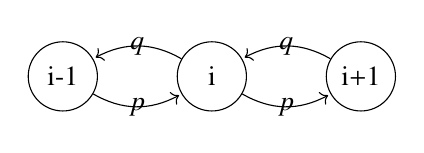
\begin{tikzpicture}
    
    \node[state]  (p) {i-1};
    \node[state,right=of p]  (q) {i};
    \node[state,right=of q]  (r) {i+1};
    \draw[every loop]
    (p) edge[bend right] node {$p $} (q)
    (q) edge[bend right] node {$q $} (p)
    (q) edge[bend right] node {$p$} (r)
    (r) edge[bend right] node {$q $} (q);
   
\end{tikzpicture}

Let $P_{i,j}^{n}$ denotes the probability of being in state j after nth transition starting from state i.
\begin{enumerate}
    \item We know that for state j in Markov chain to be \textbf{aperiodic} ,Then their  exist k such that $P_{j,j}^{n} > 0$ for all $n \geq k$. but for to return to same state j after n transitions  ,Number of forward steps should be equal to Backward steps , i.e for odd n in (2m +1)form
    \begin{align}
        P_{j,j}^{2m+1}&=0  
        \label{eq:eq1}
    \end{align}
    when n is even in 2m form
    \begin{align}
        P_{j,j}^{2m}&=\binom{2m}{m}p^{m}q^{m}
     \\
     &=\frac{(2m)!}{m!.m!}p^{m}q^{m}
     \label{eq:eq2}
    \end{align}
    ,As for odd n $P_{j,j}^{n} = 0$ ,$P_{j,j}^{n} > 0$ for all $n \geq k$ is not possible .which implies  all states are \textbf{Periodic}
  
    Option (1) is \textbf{incorrect}. 
    \item 
In a Markov Chain for state j to be recurrent then it should satisfy following condition
\begin{align}
     \lim_{t\to\infty}\sum_{n=1}^t P_{j,j}^{n}&=\infty
\end{align}
using Stirling approximation in equation \eqref{eq:eq2} 
\begin{align}
    P_{j,j}^{2m} &=\frac{((2m)^{2m +\frac{1}{2}}).e^{-2m}.(2\pi)^{\frac{1}{2}}}{m^{m+\frac{1}{2}}.e^{-m}.m^{m+\frac{1}{2}}.e^{-m}.2\pi}.p^{m}q^{m}
    \\
    &=\frac{(4pq)^{2m}}{(m\pi)^{\frac{1}{2}}}
    \label{eq:eq3}
\end{align}
In this question $p =\frac{1}{2}=q$,then using \eqref{eq:eq1} and \eqref{eq:eq3}
\begin{align}
    \lim_{t\to\infty}\sum_{n=1}^t P_{j,j}^{n}&=\sum_{n=2k,k=1}^{\infty}\frac{1}{(\frac{n}{2}\pi)^{\frac{1}{2}}}
\end{align}
Since $\frac{1}{n^{\frac{1}{2}}}$ is divergent,
\begin{align}
     \lim_{t\to\infty}\sum_{n=1}^t P_{j,j}^{n}& = \infty
\end{align}
Therefore state j is recurrent ,as what we calculated is independent of j ,all states are \textbf{recurrent }.

The first-passage-time probability, $f_{i,j}(n)$, of a Markov chain is the probability,given as 
\begin{equation}
\resizebox{.9\hsize}{!}{$f_{i,j}(n)=\pr{X_{n}=j,X_{n-1}\neq j,X_{n-2}\neq j,\dots X_{1}\neq j|X_{0}=i}$}
\end{equation}
The first-passage time $T_{j,j}$from a state j back to itself is of particular importance. It has the PMF $f_{j,j}(n)$ amd Distribution function $F_{j,j}(n)$
\begin{align}
    F_{j,j}(n)&=\sum_{k=0}^n f_{j,j}(k)
    \label{eq:eq4}
\end{align}

We Know that all states are recurrent .Now i will find whether they are null recurrent or positive recurrent .
For positive recurrent 
\begin{align}
    \overline{T_{j,j}}& < \infty
\end{align}
For null recurrent 
\begin{align}
    \overline{T_{j,j}}& = \infty
\end{align}
Where $\overline{T_{j,j}}$ is mean time to enter state j starting from j.
Now calculating $\overline{T_{j,j}}$ using below formula,
\begin{align}
    \overline{T_{j,j}}&=1 + \sum _{k=0}^n (1 - F_{j,j}(k))
    \label{eq:eq5}
\end{align}
Using \eqref{eq:eq5} and \eqref{eq:eq4},We get 
\begin{align}
    \overline{T_{j,j}}& = \infty
\end{align}
Therefore all states are null recurrent.
Option(3) is \textbf{correct}
 \item
    Since all states are recurrent,they communicate with each other ,therefore Markov chain is irreducible , option (2) is \textbf{correct}
 \item As all states are null recurrent , option (4) is \textbf{incorrect} 
\end{enumerate}
Therefore correct options are \textbf{2,3}
\end{document}
